
\documentclass{bredelebeamer}


% suppress navigation bar
\beamertemplatenavigationsymbolsempty

\mode<presentation>
{
  %\usetheme{bunsen}
  \setbeamercovered{transparent}
  \setbeamertemplate{items}[circle]
}

\beamertemplatenavigationsymbolsempty
\usepackage{color}
\definecolor{uipoppy}{RGB}{225, 64, 5}
\definecolor{uipaleblue}{RGB}{96,123,139}
\definecolor{uiblack}{RGB}{0, 0, 0}

% caption styling
\DeclareCaptionFont{uiblack}{\color{uiblack}}
\DeclareCaptionFont{uipoppy}{\color{uipoppy}}
\captionsetup{labelfont={uipoppy},textfont=uiblack}
\include{macros}

%%%%%%%%%%%%%%%%%%%%%%%%%%%%%%%%%%%%%%%%%%%%%%%%

\title[PhD]{\textbf{Applied Machine Learning with Python}}
% Titre du diaporama

\subtitle{\textbf{Part-1.Basics of Python for Machine Learning} }
% Sous-titre optionnel

\author{ \href{https://sambaiga.github.io/ }{\href{https://sambaiga.github.io/}{Anthony FAUSTINE} }}





\date{May 2017}
% Optionnel. La date, généralement celle du jour de la conférence

\subject{Sujet de votre diaporama}
% C'est utilisé dans les métadonnes du PDF



\logo{
	%
\includegraphics[scale=0.1]{images/logo.pdf}
}
\hypersetup{
	pdfauthor = {Anthony Faustine: sambaiga@gmail.com},
	pdfsubject = {},
	pdfkeywords = {},
	pdfmoddate= {},
	pdfcreator = {}
}




%%%%%%%%%%%%%%%%%%%%%%%%%%%%%%%%%%%%%%%%%%%%%%%%%%%%%%%%%%%%%%%%%%%%%
\begin{document}


\begin{frame}
	\titlepage
\end{frame}




\AtBeginSection[] { \begin{frame} %
		<beamer> \frametitle{Outline} \setcounter{tocdepth}{2} \tableofcontents[currentsection, sectionstyle=show/shaded,hideallsubsections ] \end{frame} }



%++++++++++++++++++++++++++++++++++++++++++++++++++++
\section{Python}

\begin{frame}\frametitle{Introduction}
\framesubtitle{What is Python ?}
A very popular general-purpose programming language.
\begin{itemize}
\item Open source general-purpose language
\item Dynamically semantics (rather than statically typed like Java or C/C++)
\item Interpreted (rather than compiled like Java or C/C++)
\item Object Oriented, 
\end{itemize}
\end{frame}	

\begin{frame}\frametitle{What can you use Python for?}

\begin{itemize}
\item Web development (\href{https://www.djangoproject.com/}{Django})
\item Web Scraping (\href{https://www.djangoproject.com/}{Beautiful Soup})
\item Scripting Language.
\item Scientific programming and Numeric Computing.
\item Automation and Embedded Sytstem.
\item Desktop GUIs and 3D modelling. 
\end{itemize}
\end{frame}	
	
\begin{frame}\frametitle{But Why Python ?}
\begin{multicols}{2}
\begin{figure}[h]
		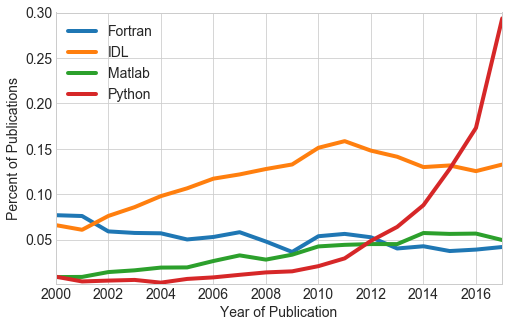
\includegraphics[scale=0.30]{../image/whypython.png}
		\label{fig:result1}
		\caption{Jake VanderPlas PyCon 2017}
\end{figure}
\columnbreak
\begin{itemize}
	\item Python is a “teaching language”
	\item ....created to “bridge the gap between the shell and C
	\item  “never intended. . . to be the primary language for programmers.”
\end{itemize}

\end{multicols}	
\end{frame}	

\begin{frame}{Why is Python such an effective tool in
science?}
\begin{enumerate}
	\item Interoperability with Other Languages
	\begin{itemize}
		\item You can use it in the shell on microtasks, or interactively, or in scripts, or to write server software, or to build enterprise software with GUIs.
	\end{itemize}	
	\item “Batteries Included” + Third-Party Modules
	\begin{itemize}
		\item Python has built-in libraries for nearly everything $\ldots$ and there are third-party
libraries for everything else.
	\end{itemize}	
	\item Simplicity \& Dynamic Nature
	\begin{itemize}
		\item  You can run your Python code on any architecture $\ldots$
	\end{itemize}	
	\item Open ethos well-fit to science
	\begin{itemize}
		\item Easy to reproduce results with python
	\end{itemize}	
\end{enumerate}	
\end{frame}


\begin{frame}{Python’s Scientific Stack}

\end{frame}	
  

\begin{frame}{Python Syntax}

\centering
{\LARGE
    Practical Session 1
}
\end{frame}

\begin{frame}{Numpy}
NumPy is the fundamental Python package for scientific computing.
\begin{itemize}
	\item Provide high-performance vector, matrix and higher-dimensional data structures.
	\item Implemented in C and Fortran for efficiency.
	\item Designed for scientific computation: linear algebra and Signal Analysis.
	\item Offers Matlab-ish capabilities within Python.
\end{itemize}	

\end{frame}	

\begin{frame}{Numpy Arrays}
NumPy provide a high-performance multidimensional array object, and tools for working with these arrays.
\begin{block}{}
\begin{itemize}
	\item A numpy array is a grid of values, all of the same type, and is indexed by a tuple of nonnegative integers.
	\item The essential difference between lists and NumPy arrays is functionality and speed.
	\begin{itemize} 
	\item Lists give you basic operation, but NumPy adds FFTs, convolutions, fast searching, basic statistics, linear algebra, histograms etc.
    \end{itemize}
    \item Thus Numpy array is memory-efficient container that provides fast numerical operations.
\end{itemize}
\end{block}	
\end{frame}	

\begin{frame}{Numpy Arrays}
\centering
{\LARGE  Practical Session 2}
\end{frame}

\begin{frame}{Matplotlib}
Matplotlib is an excellent 2D and 3D graphics library for generating scientific figures.\\
 \begin{itemize}
 	\item It provides both a very quick way to visualize data from Python and publication-quality figures in many formats.
 \end{itemize}
\end{frame}


\begin{frame}{Matplotlib}
\centering
{\LARGE  Practical Session 3}
\end{frame}



\begin{frame}{Data Analysis with Pandas}
\framesubtitle{What is pandas?}
A Python package providing fast, flexible, and expressive data structures for data analysis.
\begin{itemize}
	\item A fundamental high-level building block for doing practical, real world data analysis in Python.
	\item Designed to work with relational or labeled data or both $\Rightarrow$ a python version of Excel.
\end{itemize}	

\end{frame}


\begin{frame}{Data Analyis with Pandas}
\centering
{\LARGE  Practical Session 3}
\end{frame}


\begin{frame}{Machine Learning}
\emph{What is Machine Learning?}:The process of extracting knowledge from data automatically with the goal of making predictions or inference.\\
\begin{itemize}
	\item A classical example: Recommendations services like in Amazo or Netflix.
	\item Machine learning algorithms that learn to recognise what they see and hear are at the heart of Apple, Google, Amazon, Facebook, Netflix, Microsoft, etc.
\end{itemize}
\end{frame}

\begin{frame}{Why Machine Learning}
For many problems  it’s difcult to program the correct behavior by hand  $\Rightarrow$ with machine learning these taks are easier.
\begin{exampleblock}{Other reasons why use machine learning:}
\begin{itemize}
	\item A system might need to adapt to a changing environment.
	\item A learning algorithm might be able to perform better than its human programmers.
	\item We may want an algorithm to behave autonomously for privacy or fairness reasons.
\end{itemize}
\end{exampleblock}

\end{frame}

\begin{frame}{Type of Machine Learning}
\begin{figure}[h]
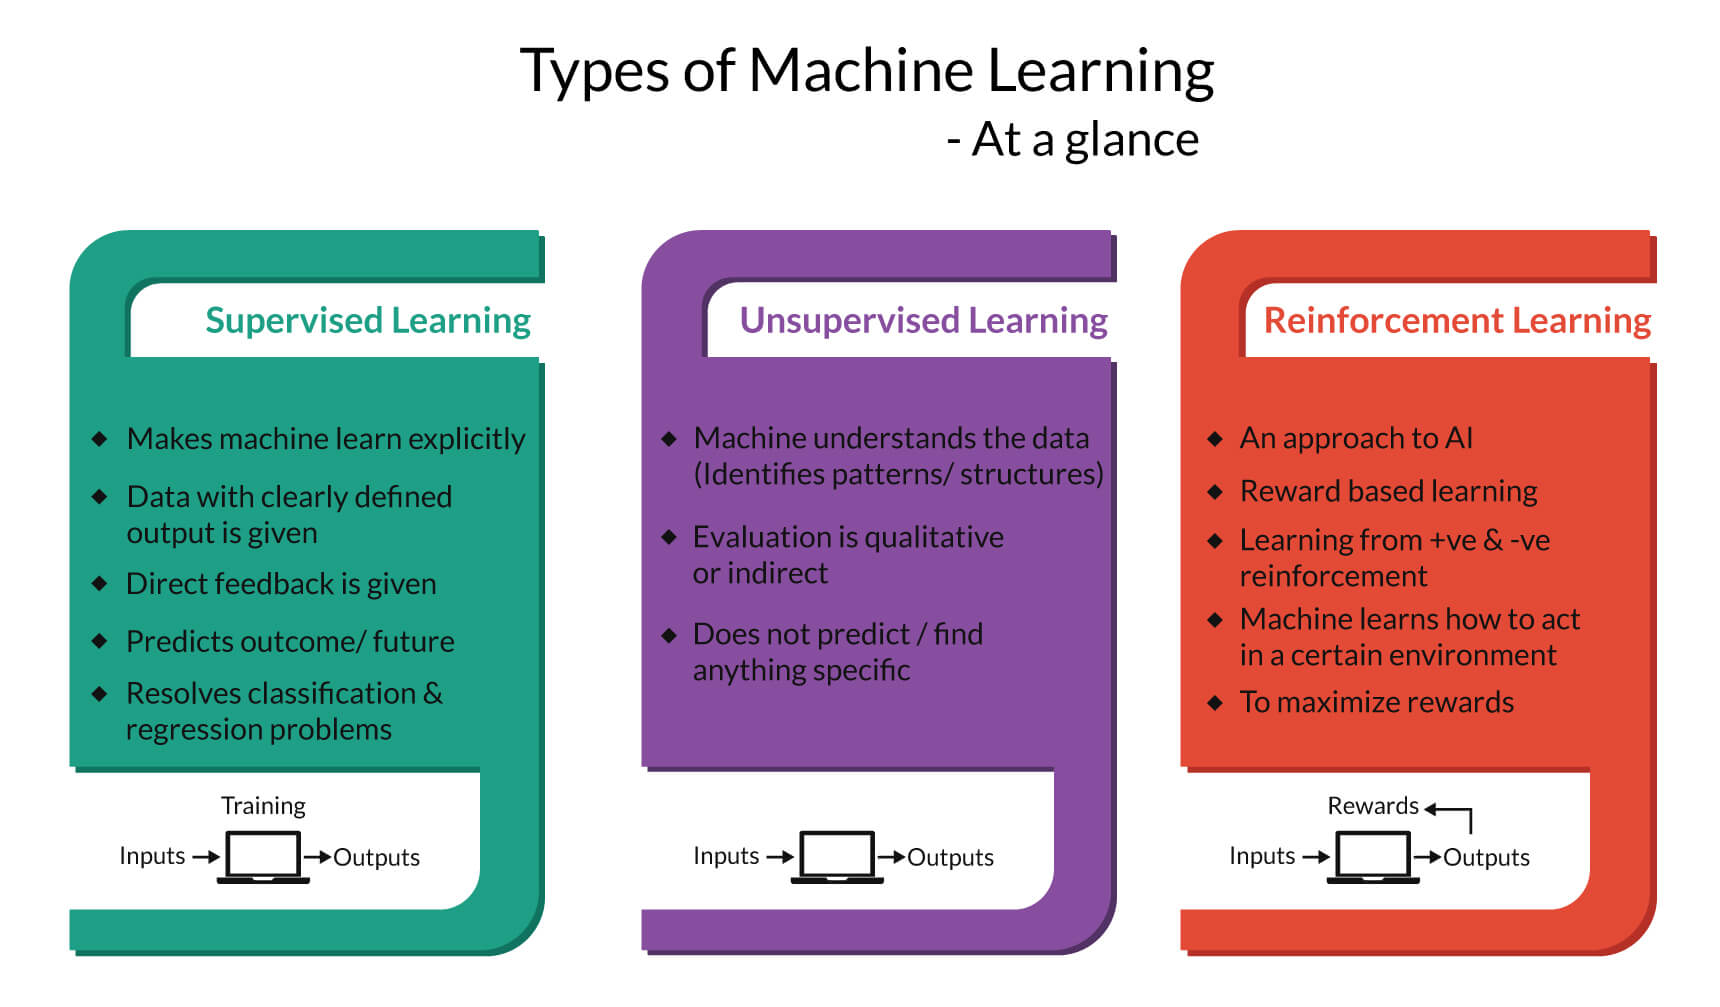
\includegraphics[scale=0.2]{../image/ml_type.jpg}
\end{figure}
\end{frame}

\begin{frame}{Type of Machine Learning}
\begin{figure}[h]
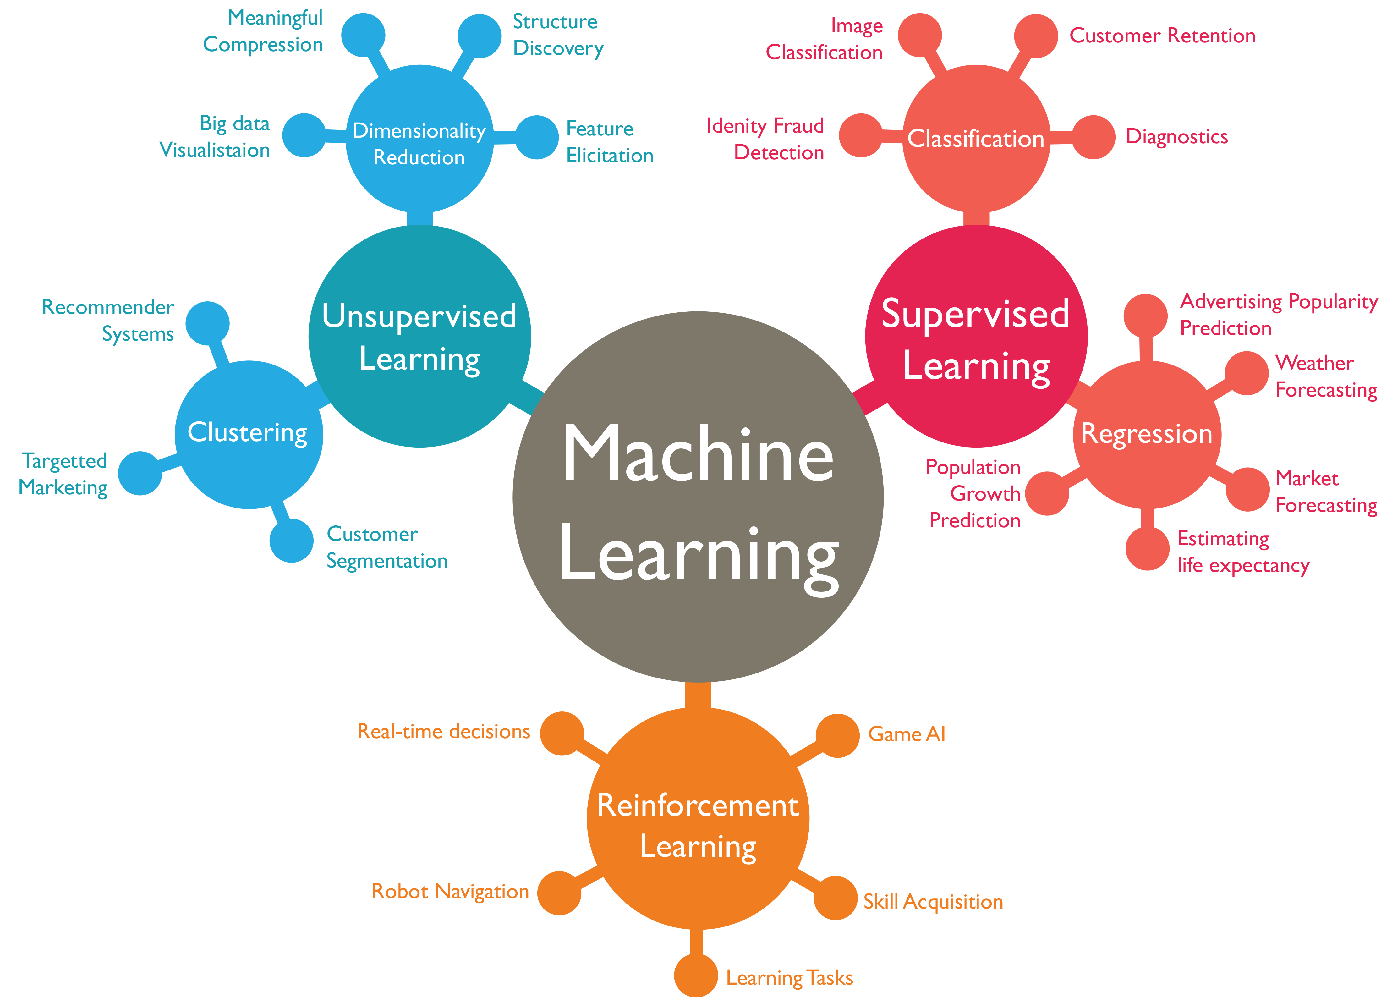
\includegraphics[scale=0.75]{../image/ml_type4.png}
\end{figure}
\end{frame}

\begin{frame}{Type of Machine Learning}
\begin{figure}[h]
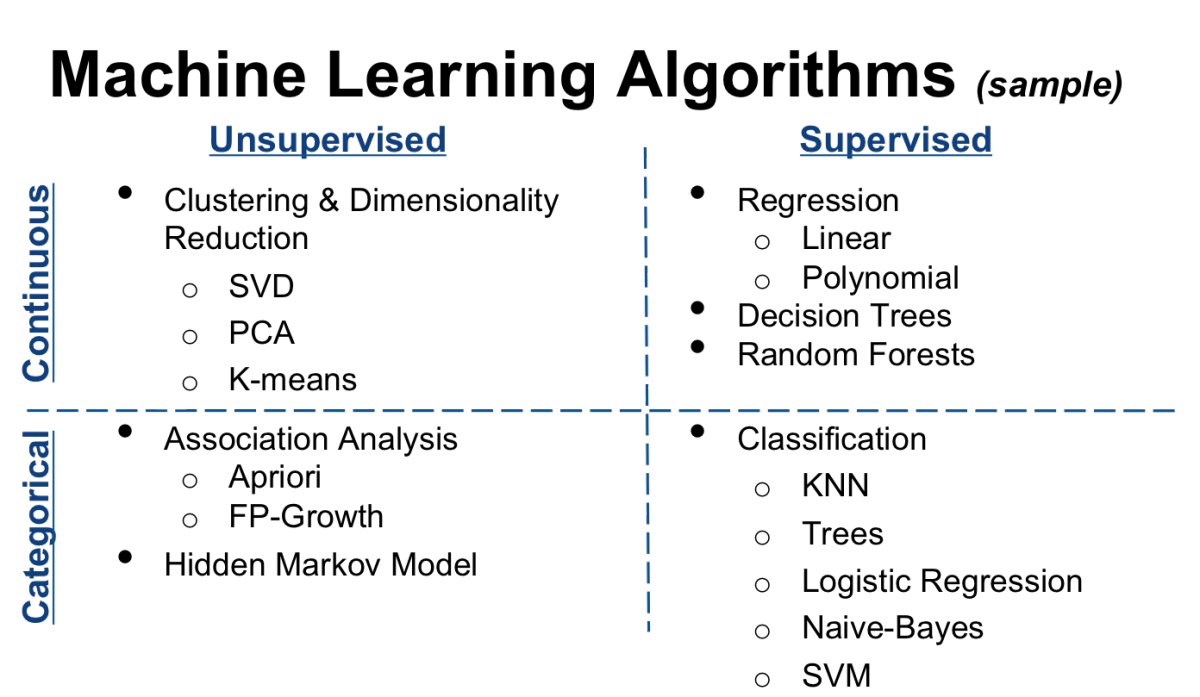
\includegraphics[scale=0.55]{../image/ml_type3.png}
\end{figure}
\end{frame}

\begin{frame}{Scikit-Learn for ML}
Scikit-Learn (sklearn) is Python's premier general-purpose machine learning library. 
\end{frame}
%-------------------------------------------------------------
\begin{frame}
\centering
\emph{THANK YOU}
\end{frame}



\end{document}

